\documentclass[14pt]{extarticle}

\usepackage[LGR]{fontenc}
\usepackage[main=greek,english]{babel}
\usepackage[utf8]{inputenc}
\usepackage[unicode]{hyperref}
\usepackage{titlepic}
\usepackage{graphicx}
\usepackage{listings}

\graphicspath{ {./img/} }

\usepackage{listings}
\usepackage{xcolor}

\hyphenpenalty=10000
\hbadness=10000

\definecolor{codegreen}{rgb}{0,0.6,0}
\definecolor{codegray}{rgb}{0.5,0.5,0.5}
\definecolor{codepurple}{rgb}{0.58,0,0.82}
\definecolor{backcolour}{rgb}{0.95,0.95,0.92}

\lstdefinestyle{mystyle}{
    backgroundcolor=\color{backcolour},   
    commentstyle=\color{codegreen},
    keywordstyle=\color{magenta},
    numberstyle=\tiny\color{codegray},
    stringstyle=\color{codepurple},
    basicstyle=\ttfamily\footnotesize,
    breakatwhitespace=false,         
    breaklines=true,                 
    captionpos=b,                    
    keepspaces=true,                 
    numbers=left,                    
    numbersep=5pt,                  
    showspaces=false,                
    showstringspaces=false,
    showtabs=false,                  
    tabsize=2
}

\lstset{frame=shadowbox, framexleftmargin=4mm, rulesepcolor=\color{black}, style=mystyle}

\title{\bfΕργασία Μεταγλωττιστών \\ Τμήμα Α2}
\titlepic{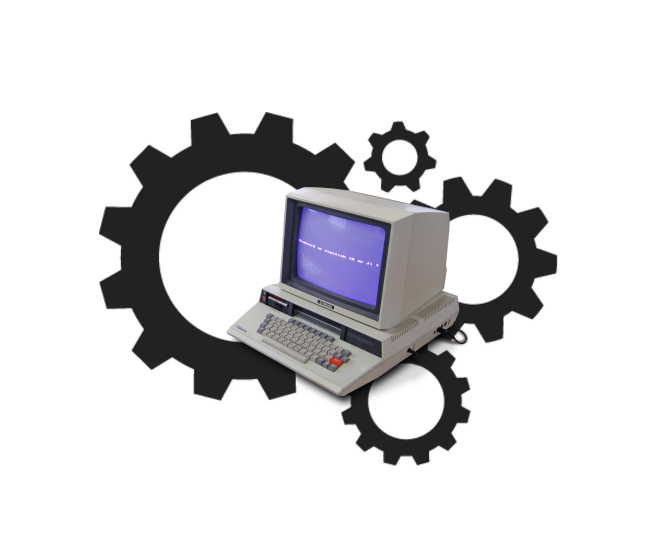
\includegraphics[scale=2.5]{computer.png}}
\author{
  \emph{Ομάδα 15}
}

\begin{document}

\begin{titlepage}
  \maketitle
  \begin{center}
    \large \emph{Ομάδα 15}
    \\
    Αναλυτικά τα μέλη:
\vspace{5mm}
  \begin{tabular}{r l}
    \\Διονύσης Νικολόπουλος & $AM: 18390126$
    \\Θανάσης Αναγνωστόπουλος & $AM: 18390043$
    \\Αριστείδης Αναγνωστόπουλος & $AM: 16124$
    \\Σπυρίδων Φλώρος & $AM: 141084$
  \end{tabular}
\vspace{5mm}
    \\
    Αναλυτικά οι ρόλοι:
    \\
\vspace{5mm}
  \begin{tabular}{r l}
    \small Γενικός Συντονιστής:   Διονύσης Νικολόπουλος
    \\
    \small Υπεύθυνος Τμήματος Εργασίας Α2: Διονύσης Νικολόπουλος
  \end{tabular}
  \\
\vspace*{\fill}
    \footnotesize{Η εργασία αυτή πραγματοποιήθηκε με χρήση \LaTeX}
  \end{center}
\end{titlepage}

\tableofcontents
\clearpage

\section{Εισαγωγή}
Στην εργαστηριακή άσκηση αυτή ασχοληθήκαμε με την δημιουργία ενός ντετερμινιστικού αυτόματου πεπερασμένων καταστάσεων.
\\
Το αυτόματο αυτό έχει ως σκοπό να λειτουργεί σαν Λεκτικός Αναλυτής της γλώσσας \textlatin{Uni-C}, ενός παρακλαδιού της γλώσσας \textlatin{C}, απο το Πανεπιστήμιο Δυτικής Αττικής.  
\\
Η κωδικοποίηση του έχει γίνει με την βοήθεια του προγράμματος \textlatin{FSM}, που επίσης είναι προγραμματισμένο πάνω στην γλώσσα \textlatin{C}. 
\clearpage

\section{Γενικευμένο Διάγραμμα Ενιαίου Αυτόματου}
\smallΕδώ είναι (γενικευμένα) το ενιαίο αυτόματο που σχεδιάσαμε:
  \begin{center}
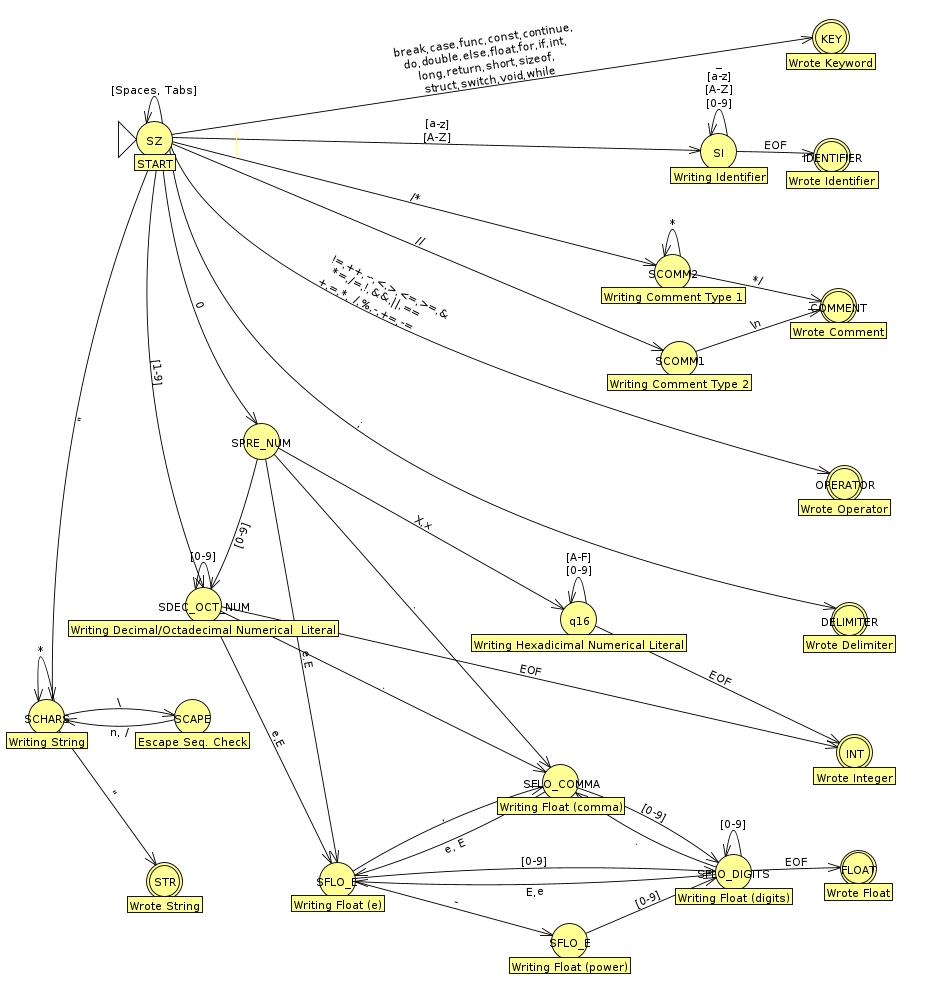
\includegraphics[scale=0.45]{automata_general.png}
  \end{center}
   
\section{Λεπτομερές Διάγραμμα Ενιαίου Αυτόματου}
\smallΕδώ είναι (γενικευμένα) το ενιαίο αυτόματο που σχεδιάσαμε:
  \begin{center}
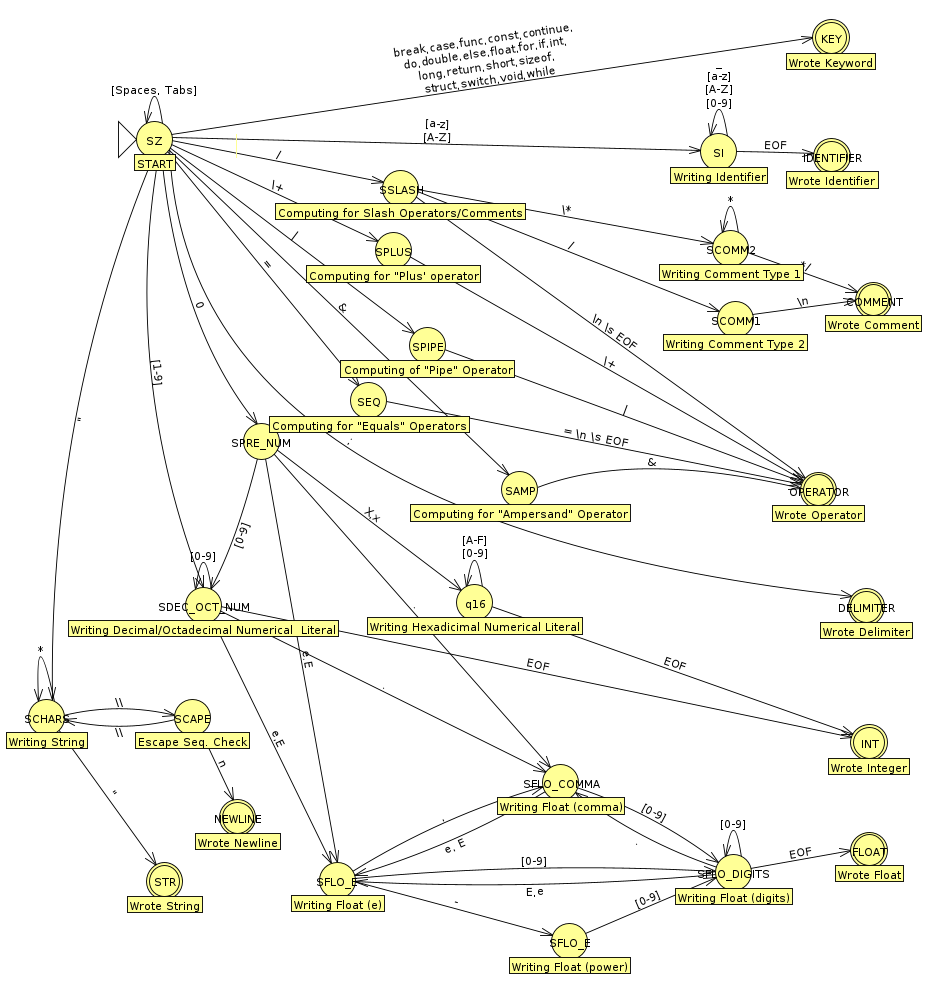
\includegraphics[scale=0.45]{automata_detailed.png}
  \end{center}

\section{Κώδικας Ενιαίου Αυτομάτου σε \textlatin{FSM}}
\small Ακολουθεί ο ολοκληρωμένος κώδικας σε \textlatin{FSM} του αυτόματού μας:  
\selectlanguage{english}
    \begin{lstlisting}
START=SZ
SZ: % -> OPERATOR
    ! < > \- = \* -> SEQ
    \+ -> SPLUS
    & -> SAMP
    ; -> DELIMITER
    | -> SPIPE
    a-z A-Z _ -> SI
    \n \s -> SZ
    / -> SSLASH
    " -> SCHARS
    0 -> SPRE_NUM
    1-9 -> SDEC_OCT_NUM
    * -> BAD


SCHARS: * -> SCHARS
        " -> STR
        \\ -> SCAPE

SCAPE:  n -> NEWLINE
        \\ -> SCHARS
        * -> BAD

NEWLINE: \s \n a-z A-Z -> SCHARS 
    
SSLASH: / -> SCOMM1
        = \n \s -> OPERATOR
        \* -> SCOMM2
    
SEQ:     = \n \s -> OPERATOR

SPLUS:   = \+  -> OPERATOR

SAMP:    & \s  -> OPERATOR

SPIPE:   |     -> OPERATOR

SI:      a-z A-Z 0-9 -> SI
         ;           -> IDENTIFIER
         \s          -> IDENTIFIER 
         EOF         -> IDENTIFIER
        
SCOMM1:     * -> SCOMM1
           \n -> SZ

SCOMM2:    \* -> SCOMM21
           * -> SCOMM2
            
SCOMM21:    / -> COMMENT

COMMENT:    \n \s -> SZ  
OPERATOR:   a-z A-Z _ -> SI
            0 -> SPRE_NUM
            1-9 -> SDEC_OCT_NUM    
            " -> SCHARS
DELIMITER:  * -> SZ
SPRE_NUM:   x X -> SHEX
            0-9 -> SDEC_OCT_NUM
            \. ->  SFLO1
            e E -> SFLO2
            
SDEC_OCT_NUM:   0-9     -> SDEC_OCT_NUM
                \.      -> SFLO_COMMA
                e E     -> SFLO_E
                \s \n ; -> FLOAT

SFLO_COMMA:     \s \n ; -> FLOAT
                e E     -> SFLO_E
                0-9     -> SFLO_DIGITS

SFLO_DIGITS:    0-9     -> SFLO_DIGITS
                \n \s ; -> FLOAT
                e E     -> SFLO_E
                \.      -> SFLO_COMMA

SFLO_E:         \.       -> SFLO_COMMA
                \-       -> SFLO_POWER 
                0-9     -> SFLO_DIGITS

SFLO_POWER:     0-9     -> SFLO_DIGITS
    
SHEX:       A-F     -> SHEX
            0-9     -> SHEX
            \s \n ; -> INT

INT:        \s \n -> SZ
            A-Z a-z _ -> SI
            % -> OPERATOR
            ! < > \- = \* -> SEQ
            \+ -> SPLUS
            & -> SAMP
            ; -> DELIMITER
            | -> SPIPE
            / -> SSLASH
            0 -> SPRE_NUM
            1-9 -> SDEC_OCT_NUM
            * -> BAD
            " -> SCHARS

FLOAT:      \s \n -> SZ
            A-Z a-z _ -> SI
            % -> OPERATOR
            ! < > \- = \* -> SEQ
            \+ -> SPLUS
            & -> SAMP
            ; -> DELIMITER
            | -> SPIPE
            / -> SSLASH
            0 -> SPRE_NUM
            1-9 -> SDEC_OCT_NUM
            * -> BAD
    
IDENTIFIER: \s \n -> SZ
            A-Z a-z _ -> SI
            % -> OPERATOR
            ! < > \- = \* -> SEQ
            \+ -> SPLUS
            & -> SAMP
            ; -> DELIMITER
            | -> SPIPE
            / -> SSLASH
            0 -> SPRE_NUM
            1-9 -> SDEC_OCT_NUM
            * -> BAD
            " -> SCHARS

STR:        \s \n -> SZ
    
BAD(OK): \n -> SZ
GOOD(OK): \n -> GOOD
    \end{lstlisting}
\end{document}
